\section{Background}
\label{sec:background}

In this section, we provide a succint summary of \ctVerif, in particular its definition of constant time (\secref{background-ct}), how the tool verifies that a program is constant-time (\secref{background-self-product}) and finally its implementation (\secref{background-tool}). 
Here we restrict ourselves to describing only those details that are needed for the rest of the report; detailed outlines of each of the above can be found in our midterm report~\cite{midterm-report}.

\subsection{Defining Constant-Time Execution}
\label{sec:background-ct}

For a program to be ``constant-time'', it must not leak any secret data that can then be identified/recovered by an adversary using timing differences. 

In their work, Almeida et. al~\cite{almeida} consider three sources of leakage:
{(1)}~branches which can leak the evaluated branch conditions, 
{(2)}~memory operations which can leak the address accessed in load and store instructions due to cache-based timing differences.
{(3)}~instructions whose execution time may vary on modern processors based on the provided operands (e.g., integer divide on x86 processors~\cite{intel-manual}). Here onwards, we refer to such instructions as ``variable latency instructions''.

In summary, Almeida et. al~\cite{almeida} define a program as constant time if it does not 
{(1)}~branch based on a secret,
{(2)}~access a secret-dependent memeory addresss, and 
{(3)}~use a secret-dependent value as an operand for variable latency instructions.
For the formal definition used by Almeida et. al~\cite{almeida}, please refer to our midterm report~\cite{midterm-report}.

%%%%%%%%%%%%%%%%%%%%%%%%%%%%%%%%%%%%%%%%%%%%%%%%%%%

\subsection{Verifying Constant-Timeliness}
\label{sec:background-self-product}

We now illustrate using an example how \ctVerif verifies that a program is indeed constant-time; \figref{example} describes the example. 
The program in question copies a sub-array of length \texttt{sub\_len}, starting at index \texttt{l\_idx}, from array \texttt{in}
to array \texttt{out}.
Both that the starting addresses and lengths of both arrays are publicly observable but the value of \texttt{l\_idx} and the array contents must be kept a secret.
Note, this program is \emph{not constant-time secure} since the branches on line 5 clearly leak information about \texttt{l\_idx}.

\begin{figure}[h]
    \centering\resizebox{0.7\columnwidth}{!}{\lstinputlisting[language=C]{example.c}}
    \caption{Running example - sub-array copy}
    \label{fig:example}
\end{figure}

To verify that a program runs in constant-time, \ctVerif verifies that its \emph{self-product} is \emph{safe w.r.t leakage assertions.}

The \emph{self-product} of a program $P$ is a second program $Q$ in which two abstract executions of $P$ take place simultaneously, with the two executions only differing in the value of \emph{secret} inputs and outputs. Said differently, $Q$ interleaves $P$ with a copy of itself and ties all public inputs of $P$ together in both executions.

\figref{example_prod} illustrates the self-product for our running example; focus now on lines $1-5$ and $12-14$. We first see that all public inputs are tied together (lines $1-4$) and assumed equal in both executions of $P$. Then both executions proceed in lock-step with each computation performed in both programs simultaneously (lines $5,12-14$).

\ctVerif utilizes the fact that the two executions differ only in the values of secret inputs to reduce constant-timeliness to safety w.r.t leakage assertions. For each of the categories of leakage it considers, \ctVerif inserts into the self-product an assertion that the leakage is the same in both executions. If the assertion holds, then the information leaked was publicly available (since only public inputs are assumed equal), if not, then the leakage differs based on the secret input which violated constant-timeliness.

\figref{example_prod} illustrates how assertion safety verifies constant-timeliness; focus now on lines $6,8,11$. Each of these three lines contain leakage assertions---line $6$ pertains to the branch on line $7$, line $8,9$ the branch on line $10$ and line $11$ the memory access on line $12$.
When a source of leakage operates only on public inputs (e.g., line $7$), the corresponding assertion holds (line $6$). 
However, when constant-time is violated and a source of leakage operates on secret-dependent values (line $10$), the corresponding assertion (line $8,9$) cannot be proved. 
Hence, if the self-product is free of leakage-assertion failures, it must be constant time.

\begin{figure}[h]
    \centering\resizebox{0.9\columnwidth}{!}{\lstinputlisting[language=MySketch]{prod.c}}
    \caption{Example program product of the sub-array copy program.}
    \label{fig:example_prod}
\end{figure}

%%%%%%%%%%%%%%%%%%%%%%%%%%%%%%%%%%%%%%%%%%%%%%%%%%%

\subsection{\ctVerif Implementation}
\label{sec:background-tool}

\ctVerif accepts two inputs---the C implementation of the program of interest and a simple proof harness which invokes the program and annotates its inputs as either public or secret.
\figref{example_wrapper} illustrates the proof harness for our running example.
Given these inputs, \ctVerif either proves that the program runs in constant time or provides sources of leakage that violate constant-time. 

\figref{ct-verif-flow} illustrates the underlying components of \ctVerif.
The program and its harness are compiled down to \codetext{llvm} bitcode. The
bitcodes are linked together and converted to \emph{Boogie Programming
Language} (\codetext{.bpl}). Compilation down to \codetext{.bpl} is automated
through \emph{SMACK}~\cite{smack}, but it is possible to customize the flow if
needed and only rely on the the \codetext{bitcode}-to-\codetext{bpl} conversion
of SMACK.
The linked \codetext{bpl} files are then fed to \emph{BAM! BAM! Boogieman} which
performs the key task of generating the self-product, and
finally the self-product---which contains assertions and assumptions---is
given to \emph{Boogie}~\cite{boogie} to verify assertion safety.

\begin{figure}[h]
    \centering
    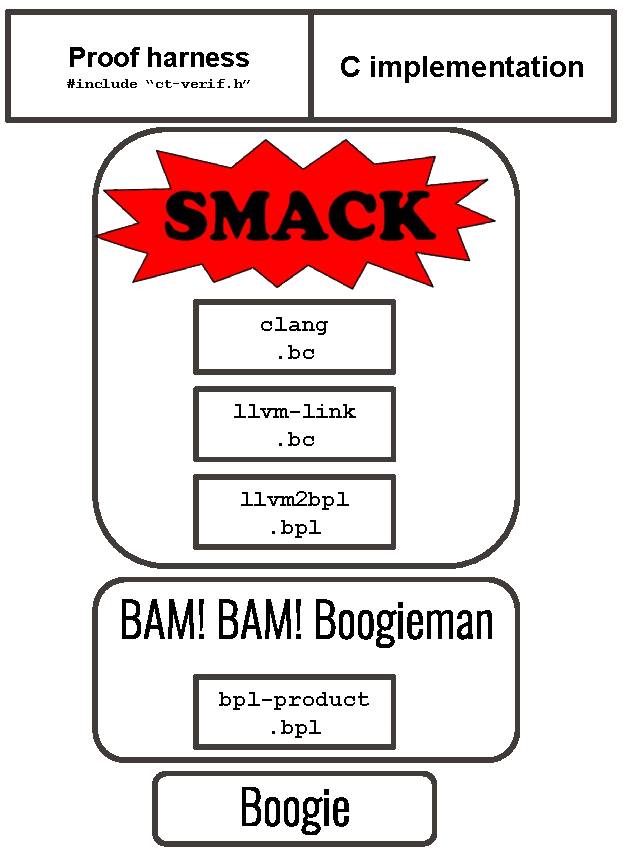
\includegraphics[height=0.4\textheight]{figs/ct-verif-flow.pdf}
    \caption{\ctVerif tool flow}
    \label{fig:ct-verif-flow}
\end{figure}

\begin{figure}[h]
    \centering\resizebox{0.7\columnwidth}{!}{\lstinputlisting[language=C]{code/example_wrapper.c}}
    \caption{Proof harness for sub-array copy in \figref{example}.}
    \label{fig:example_wrapper}
\end{figure}